\documentclass[12pt]{article}
\usepackage[british]{babel}
\usepackage{amsmath}
\usepackage{latexsym}
\usepackage{amsfonts}
\usepackage{graphicx}
\usepackage[backend=biber,style=numeric,sorting=none,isbn=false,doi=false,url=false,]{biblatex}\addbibresource{bibliography.bib}
\usepackage{subfig}
\usepackage[svgnames,table]{xcolor}
\usepackage{tikz}
%\usepackage{longtable}
\usepackage{hhline}
\usepackage{gensymb}
\usepackage{fancyhdr}
\usepackage[hidelinks]{hyperref}
%\usetikzlibrary{shapes.symbols,shapes.geometric,shadows,arrows.meta}
%\tikzset{>={Latex[width=1.5mm,length=2mm]}}
\usepackage[utf8]{inputenc}
\usepackage[T1]{fontenc}
\urlstyle{same}
\usepackage{enumitem}% http://ctan.org/pkg/enumitem
\setlist{nolistsep} % remove the vertical space altogether in all lists
\usepackage[section]{placeins}

%\let\olditemize\itemize
%\renewcommand\itemize{olditemize[noitemsep,topsep=0pt]	}

%\renewcommand{\_}{\kern-1.5pt\textunderscore\kern-1.5pt}

 %%%%%%%%%%%%  Set Depths for Sections  %%%%%%%%%%%%%%

% 1) Section
% 1.1) SubSection
% 1.1.1) SubSubSection
% 1.1.1.1) Paragraph
% 1.1.1.1.1) Subparagraph


\setcounter{tocdepth}{5}
\setcounter{secnumdepth}{5}


 %%%%%%%%%%%%  Header here  %%%%%%%%%%%%%%


\pagestyle{fancy}
\fancyhf{}
\lhead{OOGESO documentation}
\chead{}
\rhead{\thepage}
\cfoot{}
\renewcommand{\headrulewidth}{0.4pt}
\renewcommand{\footrulewidth}{0pt}

% paragraph style:
%\setlength{\topsep}{0pt}
%\setlength{\parindent}{0pt}

%\renewcommand{\arraystretch}{1.3}


%%%%%%%%%%%%%%%%%%%% Document code starts here %%%%%%%%%%%%%%%%%%%%


\author{Harald G Svendsen}
\title{Offshore Oil and Gas Energy System Optimisation (OOGESO)\\ \textbf{DOCUMENTATION}}

\begin{document}
\maketitle



\tableofcontents
%\addcontentsline{toc}{chapter}{Contents}

\newpage


\section{Introduction}
This document describes a simulation model for studying operational strategies for low-emission offshore oil and gas field energy systems (illustrated in Figure~\ref{fig:oilfield}), and the performance with different system designs.

The simulation model is being developed within the Norwegian \emph{Low Emission Research Centre}%
\footnote{\url{https://www.sintef.no/en/projects/lowemission-research-centre/}}, 
with financial support from the Research Council of Norway and Centre partners. 
The Centre aims to develop new technologies and concepts for offshore energy systems, energy efficiency and integration with renewable power production technologies for application on the Norwegian Continental Shelf.

The program code is open-source with a permissible MIT licence, and is freely available.\footnote{\url{https://bitbucket.org/harald_g_svendsen/oogeso}}


\begin{figure}
\centering
	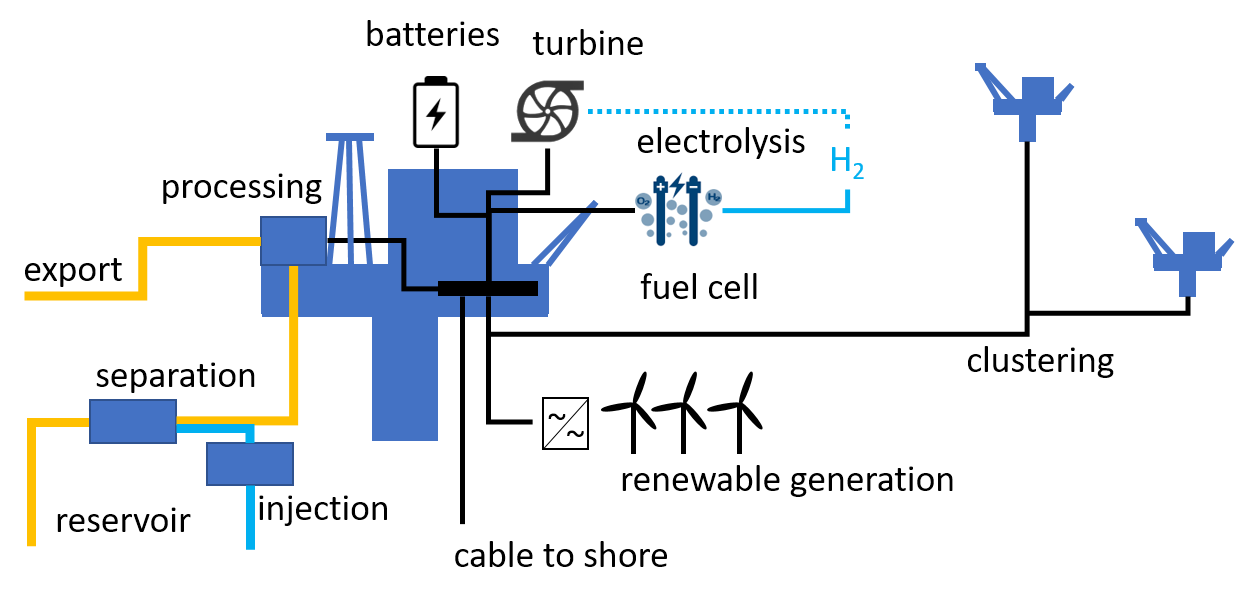
\includegraphics[width=0.8\columnwidth]{media/oilfield.png}
\caption{Offshore oil and gas field hybrid energy system}
\label{fig:oilfield}
\end{figure}



\subsection{Objective}
There are two main objectives of the hybrid energy system modelling
\begin{itemize}
	\item Compute CO2 emissions in different scenarios with different design choices and operational strategies, and compare results to provide design decision support
	\item Provide operational decision support to give economical operation with minimal CO2 emissions
\end{itemize}


\medskip\noindent
Examples of operational decisions are
\begin{itemize}
	\item Start/stop signals to gas turbines
	\item Energy storage charging and discharging signals
	\item Curtailment of wind power
	\item Power setpoint signals for flexible loads
	\item Load shedding
\end{itemize}

\medskip\noindent
Design choices that may be relevant to consider and compare include:
\begin{itemize}
	\item Power supply and energy storage options (numbers, types, capacities)
	\item Pipe dimensions and other properties
	\item Device parameters (e.g. ramp rate and capacity of gas turbine)
	\item Amount of load flexibility
\end{itemize}

\medskip\noindent
Operational strategy is encoded in the problem formulation indirectly through
\begin{itemize}
	\item Strategy for storage utilisation
	\item Risk tolerance level
	\item Forecasting
	\item Parameter choices (e.g. allowable max/min bounds).
\end{itemize}

%Expand to use as operational decision support? Forecasting energy demand, energy availability (wind) and optimise dispatch. Should gas turbine be started up? – multi-horizon optimisation




\section{Model concepts}

This chapter provides a high-level description of the underlying concepts applied in the model. More details are given in chapters \ref{sec:networks} and \ref{sec:devices}.


\subsection{Optimisation problem}

The purpose of this software tool is to provide operational decision support for an offshore energy system with a specified configuration.  Specifically, the task is to provide set-points for controllable variables in the system to minimise CO\textsubscript{2} emissions as well as costs for fuel and costs associated with lost oil/gas export. 
The main controllable variables are power output of generators, power demand of flexible loads, charging and discharging of energy storages. This is therefore an optimisation problem with an objective function given by weighing between CO\textsubscript{2} emissions and costs, and constraints that represent inter-dependencies and bounds. For example, the relationship between pressure drop and energy flow in a gas pipe is represented by an equation that is a constraint in the optimisation problem. Another example is the relationship between gas consumption and electric power and heat output of a gas turbine generator.

The problem includes \emph{integer} variables representing start/stop status of devices. For solvability, the problem is \emph{linearised}, i.e. objective function and constraints are linear expression with respect to the variables. The optimisation problem therefore classifies as a mixed-integer linear programming (MILP) problem.


\subsubsection{Time-steps and horizons}

For operational control and CO2 emission estimation, the variability with time of energy demand and energy availability is important, as are start-up costs and ramp rate limitations of turbines, and possibly other device types. Time variability is included via time-series and time-step by time-step solutions of the problem.

For the planning of start-up and shut-down of devices, notably gas turbines operated in combination with wind power supply, it is necessary to consider a time-horizon stretching into the future rather than just the present time snapshot. If wind power is rapidly dropping and an extra gas turbine is required at full power in 2 hours, the gas turbine may have to be started already now because of ramp rate limits. And instead of shutting down the gas turbine for one hour, and then starting it up again, it may be more economical to keep it running (to avoid start-up costs). Optimal charging and discharging of battery, and utilisation of demand flexibility likewise depends on what is expected to happen next.

As an operational planning tool, therefore, the model contains a rolling horizon optimization, where the system is optimised for a certain planning horizon that is continuously shifted forward, see Figure~\ref{fig:rollinghorizon}. For example. The optimisation may be done for every 15 minutes for the next 12 hours, repeated at every hour.

\begin{figure}
\centering
	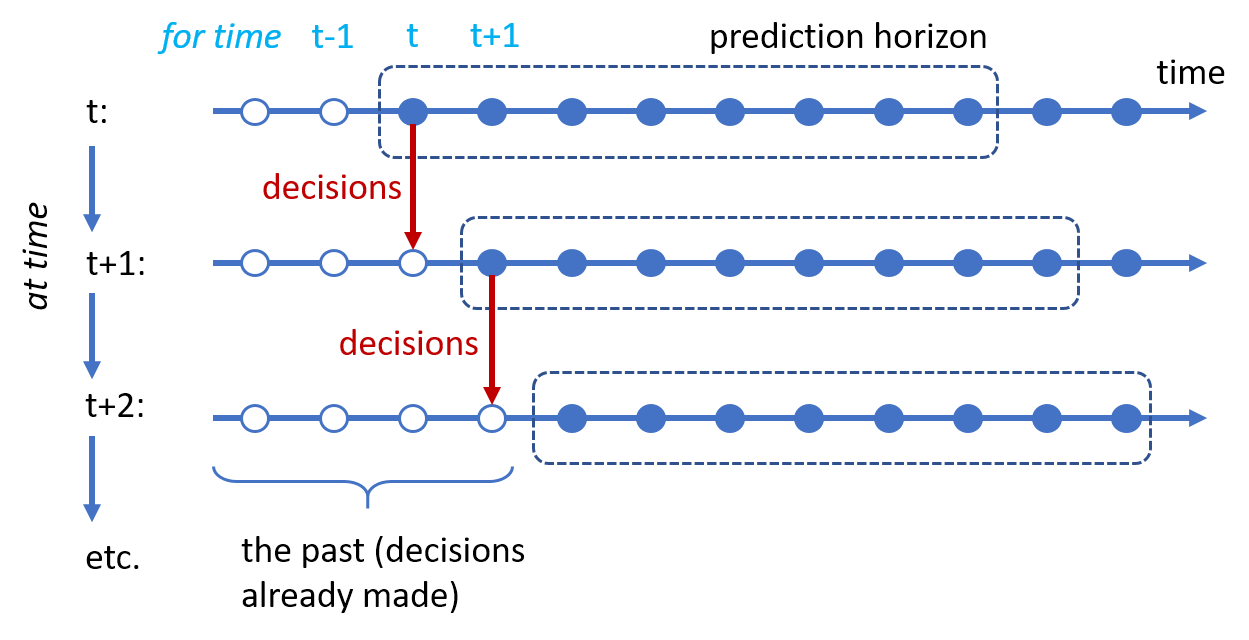
\includegraphics[width=\columnwidth]{media/optimisation_rollinghorizon.png}
\caption{Rolling horizon optimization}
\label{fig:rollinghorizon}
\end{figure}


\subsection{Energy carrier networks}

The offshore energy system is modelled as a hybrid system with multiple energy carriers, see Figure~\ref{fig:energy_system}.
There are energy transfer links or \emph{networks} for each energy carrier,
 and \emph{devices} that consume, produce, or convert energy from one form to another.


Networks are modelled for the different energy carriers. Network topology is specified by sets of nodes and edges. An edge is a connection between two nodes.


\begin{figure}
\centering
	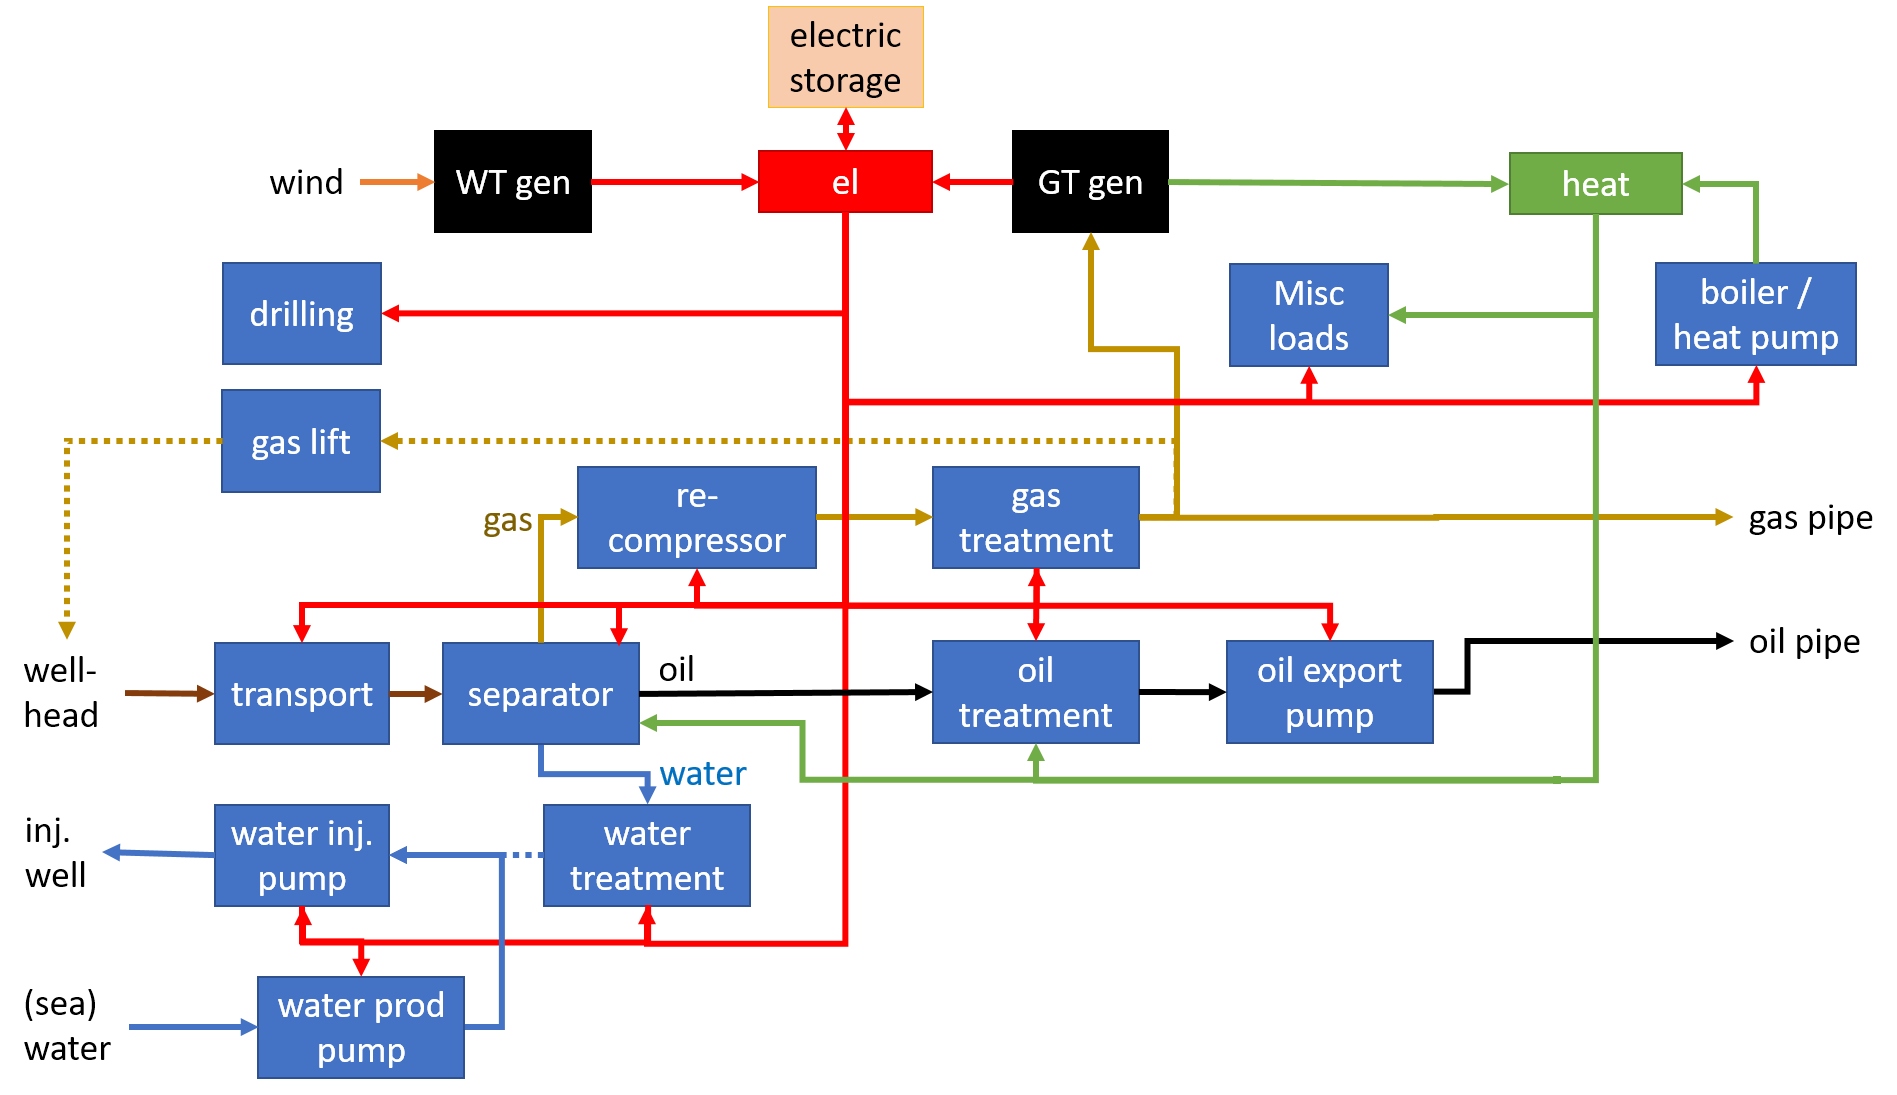
\includegraphics[width=\columnwidth]{media/energy_system.png}
\caption{Example schematic of an offshore multi-carrier hybrid energy system}
\label{fig:energy_system}
\end{figure}


\subsubsection{Network components}

\begin{description}
\item[Nodes]
Connection points for devices and edges. A node has input/output terminals (see below) for different energy carriers. 

\item[Terminals]
Terminals exist within a node. There are different terminals for the different energy carriers. If there are \textit{series} connected devices, the terminal is split in an \textit{in} terminal and an \textit{out} terminal. Edges and devices are linked to specific terminals within a node.

\item[Edges]
Connection between nodes, with physical properties depending on network type. Energy flows through the edges.

\item[Devices]
Things that "do" something in the network. Consumption and generation of one or more of the energy carriers. Devices are modelled as either
\begin{itemize}
	\item consumer/producer – these are devices that extract and/or inject power into of one or more energy carriers. Examples: gas turbine, electric auxiliary load, water injection pump, ...
	\item series devices – these are devices with power flowing through with an input terminal and an output terminal with different properties (e.g. gas pressure). Examples: oil pumps, gas compressors
\end{itemize}
More information about device modelling is given in Section \ref{sec:devices}.
\end{description}

\subsubsection{Energy carriers and network types}

The energy carriers and their most relevant network properties/characteristics are:
\begin{description}
	\item[Electricity] Electric power through electric conductors
	\begin{itemize}
		\item impedance, energy loss, max flow, 2-directional
		\item power flow determined by endpoint voltage angles
	\end{itemize}
	\item[Heat] Thermal energy transport
	\begin{itemize}
		\item modelled as lossless energy transfer (assuming short distances)
	\end{itemize}
	\item[Wellstream] Raw crude oil through pipelines
	\begin{itemize}
		\item pressure, viscosity, 1-directional
		\item composition (oil/gas/water) of wellstream is highly case-dependent
	\end{itemize}
	\item[Gas] Gas through pipelines
	\begin{itemize}
		\item pressure, diameter, friction, gas properties, 1-directional
		\item flow determined by endpoint pressure and pipeline friction
	\end{itemize}
	\item[Oil/water] Liquid oil and water through pipelines
	\begin{itemize}
		\item pressure, diameter, friction, fluid properties, 1-directional
		\item flow determined by endpoint pressure and pipeline friction
	\end{itemize}
\end{description}
The raw wellstream flowing from the well is considered a mix of oil, gas and water, with composition ratio specified as input.



\subsection{Devices}

Detailed description of the various device types are given in Section~\ref{sec:devices}, but some common, generic concepts are described in the following.


\subsubsection{Upper and lower bounds}

Typically the energy or volume flow rate ($P$ or $Q$) in or out of devices are limited by maximum and minimum values (provided as user input). Sometimes these bounds are time-dependent. For example, for wind power the maximum electrical output is limited by available wind power.

\begin{equation}
	 P_{\min } \leq P_{device} \leq p(t) P_{\max } 
\end{equation}
The function $p(t)$ is a time profile that may be specified to represent e.g. wind power availability. 
If no time profile is specified in the input,  $p(t)=1$  is used.


\subsubsection{Ramp rate limits}
Devices may have ramp rate limits defined, and exactly what is limited varies slightly between different device models.  Typically this is electric power input or output, or heat output:
\begin{equation}
	 \text{maxRampDown} \leq P_{t}-P_{t-1} \leq  \text{maxRampUp}
\end{equation}


\subsubsection{Flexibility}

An important aspect of the integrated modelling of the system is the analysis of the impact and benefit of flexibility such as the option of adjusting water injection in response to available wind power.


Flexibility is included in the model by introducing an energy buffer that allows power demand to deviate from the nominal or average value. Mathematically, this is very similar to the modelling of energy storage. 




\subsubsection{Optimisation variables}

Associated with devices are the following variables:
\begin{itemize}
	\item device flow(\texttt{varDeviceFlow}) – power/volume flow per carrier, in and out of the device
\end{itemize}
%
For devices with start-up time delay or costs, the following variables are used:
\begin{itemize}
	\item on/off status (\texttt{varDeviceIsOn})– binary variable indicating if device is online
	\item startup (\texttt{varDeviceIsPrep}) – binary variable indicating if device is in startup phase (preparing to go online)
	\item starting (\texttt{varDeviceStarting}) – binary variable indicating if device is started (activated)
	\item stopping (\texttt{varDeviceStopping}) – binary variable indicating if device is stopped
\end{itemize}
%
And for devices with energy storage:
\begin{itemize}
	\item device energy storage level (\texttt{varDeviceEnergy}) – state of charge for associated energy storage
	\item device energy storage power available (\texttt{varDeviceEnergyPower}) – available power from storage in a given timestep
\end{itemize}


Section~\ref{sec:devices} gives an overview of the various implemented device types.




%%%%%%%%%%%%%%%%%%%%%  Networks  %%%%%%%%%%%%%%%%%%%%%%%%%%%%

\section{Energy carrier networks}
\label{sec:networks}

This chapter describes in more detail the modelling of energy flow in the different types of networks.


\subsection{Electricity network}

Alternating current (AC) power flow in an electricity network is governed by non-linear power flow equations which express the relationships between line impedances (physical properties), complex net power injections, and voltage angle and magnitude at each node. Power flow is derived from voltage angle differences


The\ electricity network for offshore energy systems (platform or cluster of platforms) is a type of distribution grid with voltage levels from 230 V to 20 kV, potentially higher for interconnections. The network normally has a radial structure.  There are three main modelling alternatives
\begin{itemize}
	\item Energy transport model
\begin{itemize}
	\item power flow only limited by line capacity limits
	\item voltages ignored; only active power considered

\end{itemize}
	\item Linearised power flow model (DC power flow)
\begin{itemize}
	\item power flow determined by linearised power flow equations
	\item line flow limited by line capacity 
	\item assumes voltage magnitudes at nominal values, ignores reactive power flow

\end{itemize}
	\item Non-linear power flow model (AC power flow) (not implemented)
\begin{itemize}
	\item computes active and reactive power flow, voltage magnitude and angle
\end{itemize}
\end{itemize}




\noindent
Constraints:
\begin{itemize}
	\item Power flow balance at each node (power flow equations)
	\item Limits on transmitted power in edges
	\item Voltage limits at nodes
\end{itemize}


\subsection{Gas network (pipelines)}

Energy flow in the gas pipeline network is modelled using linearised Weymouth equations, as outlined in the following. 
Symbols are defined in Table~\ref{tab:gasnetworksymbols}.

The flow equation relates gas flow and pressure. Mass conservation means that the mass flow (measured in kg/s) is constant throughout a pipe with fixed diameter, whereas the volumetric flow (measured in m\textsuperscript{3}/s) depends on the pressure, flow increases when pressure decreases (gas particles require more space). Mass and volumetric flow are related via the pressure:
\begin{equation}
	W= \rho _{in}Q_{in}= \rho _{out}Q_{out}= \rho _{s}Q. 
\end{equation}


The subscript \textit{s} denotes standard conditions (temperature  \( T_{s}=273.15 \)  K and pressure  \( p_{s}=100 \)  kPa). The density  \(  \rho _{s} \)  is a fixed value but  \(  \rho _{in} \)  and  \(  \rho _{out} \)  depend on the pressure and temperature. The below gas flow equations are expressed using standard condition flow rate  \( Q \) . As mass flow, this is the same at any point on the pipe.


For a gas, the density depends on the pressure. Assuming ideal gas, this relationship is 
\begin{equation}
	p_{i}= \rho _{i}\frac{R}{M}T_{i}, 
\end{equation}
%
where  \( R=8.314\frac{J}{\text{mol K}} \)  is the universal gas constant,  \( M \)  is the molar mass (kg), and  \( T \)  is the temperature (K). For natural gas, the molar mass is  \( M=0.019 \)  kg/mol. Thus,  
\(  \rho _{s}=\frac{Mp_{s}}{RT_{s}}=0.84\frac{kg}{m^{3}}~. \) 



\begin{table}[]
\caption{Symbols used in gas network modelling}
\label{tab:gasnetworksymbols}
\begin{tabular}{llp{12em}p{8em}}
\hline 
symbol         & unit   & description                                           & value                      \\
\hline
$Q_d$          & m3/day & gas flow rate, standard conditions                    & (computed)                 \\
$Q$            & m3/s   & gas flow rate, SI units, standard conditions          & (computed)                 \\
$W$            & kg/s   & mass flow rate                                        &                            \\
$P$            & MW     & energy flow                                           & (computed)                 \\
$CV$           & MJ/m3  & energy value (calorific value) at standard conditions & 40 MJ/m3 for natural gas   \\
$T_b$          & K      & base temperature, ambient temperature?                & 273+15 K                   \\
$p_b$          & kPa    & base pressure, local atmospheric pressure             & 101 kPa (1 bar)            \\
$p_\text{in}$  & kPa    & pipe pressure inlet                                   &                            \\
$p_\text{out}$ & kPa    & pipe pressure outlet                                  &                            \\
$L$            & km     & pipe length                                           &                            \\
$\rho_s$       & kg/m3  & gas density, standard conditions                      & 0.84 kg/m3 for natural gas \\
$T_f$          & K      & gas temperature                                       &                            \\
$G$            & 1      & gas gravity (air = 1)                                 & 0.6 ?                      \\
$Z$            & 1      & compressibility factor                                & 0.9 ?                      \\
$f$            & 1      & Darcy friction factor                                 & (computed)                 \\
$D$            & mm     & pipe inside diameter                                  & 150–1200 ??                \\
$h_\text{in}$  & m      & height inlet                                          &                            \\
$h_\text{out}$ & m      & height outlet                                         &                            \\
$s$            & 1      & elevation factor                                      & (computed)                 \\
$L_e$          & km     & equivalent length                                     & (computed)    \\
\hline            
\end{tabular}
\end{table}




There are several different approximations describing the gas flow in a gas pipeline network\footnote{ E Sashi Menon, Gas Pipeline Hydraulics, Taylor $\&$  Francis (2005), https://doi.org/10.1201/9781420038224  }. The general flow equations, expressing the gas volumetric flow rate (under standard conditions)  \( Q_{d} \)  from high to low pressure ( \( p_{in} \geq p_{out} \) ) is
\begin{equation}
  Q_{d}=1.1494 \times 10^{-3}\frac{T_{b}}{P_{b}}\sqrt[]{\frac{ \left( p_{in}^{2}-p_{out}^{2} \right) }{GT_{f}LZf}}D^{5/2}= \left(  \ldots  \right) \sqrt[]{ \left( p_{in}^{2}-p_{out}^{2} \right) }, 
\end{equation}
%
The Darcy friction factor  \( f \)  is sometimes replaced by  \( F=2/\sqrt[]{f} \)  (transmission factor). 


Including elevation difference, the equation becomes
\begin{equation}
  Q_{d}=1.1494 \times 10^{-3}\frac{T_{b}}{P_{b}}\sqrt[]{\frac{ \left( p_{in}^{2}-e^{s}p_{out}^{2} \right) }{GT_{f}L_{e}Zf}}D^{\frac{5}{2}} 
\end{equation}


The factor  \( e^{s} \)  and the equivalent length  \( L_{e} \)  together account for elevation differences. These are defined as:
\begin{equation} 
	s=0.0684 G\frac{h_{2}-h_{1}}{T_{f}Z}, 
\end{equation}
\begin{equation}
	 L_{e}=L\frac{e^{s}-1}{s}, 
\end{equation} 
where  \( h_{} \)  is elevation (in m) and  \( L \)  is the segment length (km).


Using for the friction factor  \( F=6.521D^{1/6} \) , or equivalently,  \( f=\frac{4}{F^{2}}=0.09406 D^{-1/3} \) , we get the (non-linear) Weymouth equation:
\begin{equation}
	 Q_{d}=3.7435 \cdot 10^{-3}\frac{T_{b}}{P_{b}}\sqrt[]{\frac{ \left( p_{in}^{2}-e^{s}p_{out}^{2} \right) }{GT_{f}L_{e}Z}}D^{\frac{8}{3}}. 
\end{equation} 


In our model, we base the description on the Weymouth equation, which is appropriate for high pressure, high flow rates and large diameter gas pipelines. 


The flow rate  \( Q \)  in standard SI units (m3/s) is:
\begin{equation}
 	 Q=\frac{\text{1 day}}{24 \cdot 3600 s}Q_{d}=k\sqrt[]{ \left( p_{in}^{2}-e^{s}p_{out}^{2} \right) }, 
\end{equation} 




where the constant  \( k \)  is a property of the pipeline and the gas, given as 
\begin{equation}
 	k=4.3328 \cdot 10^{-8}\frac{\mathrm{m}^{\mathrm{3}}}{\mathrm{\text{s MPa}}} \cdot  \frac{T_{b}}{P_{b}} \left[ GT_{f}L_{e}Z \right] ^{-\frac{1}{2}}D^{\frac{8}{3}}, 
\end{equation}
%
where quantities are expressed in units [T]=K, [P]=MPa, [L]=km, [D]=mm. 

\subsubsection{Linearisation}

Assuming that the pressure remains close to the given nominal values  \( p_{in,0}^{} \)  and  \( p_{out,0}^{} \)  at the pipe endpoints, we can linearise the Weymouth equation by expanding around these values\footnote{ A Tomasgard et al., Optimization\  models\ \ for\ \ the\ \ natural  gas  value  chain, in: Geometric Modelling, Numerical Simulation and Optimization. Springer Verlag, New York (2007), https://doi.org/10.1007/978-3-540-68783-2\_16  }:
\begin{equation}
 	 p_{in}=p_{in,0}^{}+ \Delta p_{in},~~p_{out}=p_{out,0}^{}+ \Delta p_{out}
\end{equation}
%
This gives the following linear approximation:
\begin{equation}
	Q\simeq\frac{k}{\sqrt[]{ \left( p_{in,0}^{2}-e^{s}p_{out,0}^{2} \right) }} \left[ p_{in,0}p_{in}-e^{s}p_{out,0}p_{out} \right] 
\end{equation}
(if  $p_{out}$ is smaller, $Q$ is larger). 
Note: This approximation is only valid if  \( p_{in} \approx p_{in,0}^{} \)  and  \( p_{out} \approx p_{out,0}^{} \) .
To determine appropriate nominal pressure values, the non-linear Weymouth equation may be used to compute the pressure drop in a pipe for the expected flow rate.

\medskip\noindent
Constraints:
\begin{itemize}
	\item Energy balance at each terminal 
	\item Limits on pressure deviation from nominal value
	\item Edge flow vs terminal pressure (Weymouth equation)
\end{itemize}

\subsubsection{Volumetric flow vs energy flow}
The energy flow ($P$) is given by the standard condition volume flow ($Q$) and the gas energy value (calorific value),  $CV$ : 
 \begin{equation}
 	 P=Q \cdot CV 
\end{equation}
The units are MW for energy flow, m\textsuperscript{3}/s for volume flow and MJ/m\textsuperscript{3} for the energy value.




\begin{table}[]
\caption{Symbols used in liquid pipeline modelling}
\label{tab:oilpipe}
\begin{tabular}{llp{15em}l}
\hline
symbol        & unit     & description                              & value                         \\
\hline
$Q$           & m3/s     & liquid flow rate, SI units               & (computed)                    \\
$P$           & MW       & energy flow                              & (computed)                    \\
$CV$          & MJ/m3    & energy value (calorific value)           & 36000 MJ/m3 for raw oil       \\
$f$           & 1        & Darcy friction factor                    & 0.008 – 0.10                  \\
$z$           & m        & elevation at inlet and outlet            &                               \\
$p$           & Pa       & pressure at inlet and outlet             &                               \\
$\rho$        & kg/m3    & fluid mass density (water: 1000 kg/m3)   & oil: 900                      \\
$L$           & m        & pipe length                              &                               \\
$D$           & m        & pipe internal diameter                   & 0.2                           \\
$e$           & m        & absolute pipe roughness                  &                               \\
$ \langle V \rangle$         & m/s      & average liquid velocity                  & oil: 2.5, gas: 15             \\
$g$           & m/s2     & gravitational acceleration               & 9.98                          \\
$\nu$         & m2/s     & fluid kinematictic viscosity             & brent: 2.86e-6 at 50\degree C        \\
$\mu=\nu\rho$ & kg/(m s) & fluid viscosity (depends on temperature) & oil: ca 0.0026, water: 0.0010 \\
Re            & 1        & Reynolds number                          & oil: 1.75e5        \\
\hline          
\end{tabular}
\end{table}




\subsection{Liquid flow network (oil and water)}

The mass or energy flow from the well, oil and water is modelled as the flow of incompressible fluids as follows.
Symbols used are defined in Table~\ref{tab:oilpipe}.

The pressure loss (head loss) in an incompressible fluid (liquid) pipeline due to friction is described by the empirical Darcy-Weisbach equation\footnote{ E Shashi Menon, Liquid Pipeline Hydraulics, CRC Press (2004), https://doi.org/10.1201/9780203021385  } (with the effect of elevation difference ( \( z \) ) included),
 \begin{equation}
 \Delta p=p_{out}-p_{in}
 	=- \rho g \left( z_{out}-z_{in} \right) -f\frac{ \rho L}{D}\frac{ \langle V \rangle ^{2}}{2}, 
 \end{equation}
where symbols are explained in Table 2. Since the velocity  \(  \langle V \rangle  \)  is related to the volumetric flow rate ( \( Q \) ),


 \begin{equation}
 Q=A \langle V \rangle 
 	=\frac{ \pi D^{2}}{4} \langle V \rangle  \Longrightarrow   \langle V \rangle ^{2}
 	=\frac{16~Q^{2}}{ \pi ^{2}D^{4}}, 
 \end{equation}
we can write
\begin{equation}
	p_{out}-p_{in}=- \rho g \left( z_{out}-z_{in} \right) -\frac{8f \rho LQ^{2}}{ \pi ^{2}D^{5}}. 
\end{equation}
Or the equation can be inverted to give the flow rate in terms of pressure:
\begin{equation}
 Q=\sqrt[]{\frac{ \pi ^{2}D^{5}}{8f \rho L}}\sqrt[]{p_{in}-p_{out}- \rho g \left( z_{out}-z_{in} \right) } 
\end{equation}
 
\textit{Example}: Friction factor  $f=0.01$, density  $\rho=900$~kg/m3, diameter  $D=0.2$~m, 
flow rate  $Q=0.1$~m3/s, and no height difference, gives pressure drop  $\Delta p/L=0.22$~MPa/km.


\subsubsection{Darcy friction factor}
The Darcy friction factor  \( f \)  depends on pipe properties. First, the Reynolds number is defined as 
\begin{equation}
	 Re=\frac{ \rho  \langle V \rangle D}{ \mu }=\frac{ \langle V \rangle D}{ \nu }.
\end{equation} 
%
There are three flow regimes, depending on the Reynolds number:
\begin{itemize}
	\item laminar, Re < 2000
	\item critical, 2000 < Re < 4000
	\item turbulent, Re > 4000
\end{itemize}


For laminar flow (Re<2000), the friction factor depends only on the Reynolds number, and not e.g. on the internal smoothness of the pipe. This is referred to as the Moody friction factor:
 \[ f=f_{\mathrm{Moody}}=\frac{64}{Re}. \] 
However, for oil pipes, flow velocity is typically so high that the flow is turbulent. In this case (Re>4000), the friction factor is given by the phenomenological \textit{Colebrook-White} equation:
 \[ \frac{1}{\sqrt[]{f}}=-2\log _{10} \left( \frac{e}{3.7D}+\frac{2.51}{Re\sqrt[]{f}} \right) . \] 
In smooth pipes, the roughness term may be neglected, giving the \textit{Kármán–Prandtl} resistance equation:
 \[ \frac{1}{\sqrt[]{f}}=-2\log _{10} \left( \frac{2.51}{Re\sqrt[]{f}} \right) =2\log _{10} \left( Re\sqrt[]{f} \right) -0.8. \] 


Another set of coefficients for this equation sometimes used is:
 \[ \frac{1}{\sqrt[]{f}}=1.930\log  \left( Re\sqrt[]{f} \right) -0.537=0.838 W \left( \text{0.629 Re} \right) , \] 


where  \( W \)  is the Lambert W function. The friction factor changes by about one order of magnitude for a five orders of magnitude change in Reynolds number: \textit{Re}=4000 gives \textit{f}=0.039, whereas \textit{Re}=10\textsuperscript{8} gives \textit{f}=0.006.


Knowing the volumetric flow rate ( \( Q \) ), the fluid density ( \(  \rho  \) ) and viscosity ( \(  \mu  \) ), and pipe internal diameter ( \( D \) ), the Reynolds number is given as
 \[ Re=\frac{ \rho }{ \mu } \langle V \rangle D=\frac{2}{ \pi }\frac{ \rho Q}{ \mu D}. \] 
Note that  \(  \rho Q \)  equals the mass flow rate (kg/s)


\medskip\noindent
\textit{In our model, it is assumed that the friction factor is provided as user input for each oil pipe. Differences in friction factor due to changes in the flow rate and temperature (affecting viscosity) are ignored.}


\textit{Example:}
Assume  \( Q= \) 1.85 Sm3/s,  \(  \rho = \) 900 kg/m3), giving \(  \rho Q=1666 \)  kg/s,  \(  \mu =3 \) ,  \( D=0.1 \)  m gives  \( Re=5300 \) , which in turn gives \textit{f} = 0.036.
 \(  \rho Q=1666 \)  kg/s,  \(  \mu =0.003 \) ,  \( D=0.1 \)  m gives  \( Re=3.5e6 \) , which in turn gives \textit{f} = 0.0097.



\subsubsection{Linearisation of equation (UPDATE)}
Since the pressure drop depends on the square of the flow rate, the above Darcy-Weisbach is non-linear and must be linearised to give linear constraint equations. Let the operating point be defined by pressure levels and flow rate  \( p_{in,0},~p_{out,0},~Q_{0} \) :
\begin{equation}
	 Q_{0}=\sqrt[]{\frac{ \pi ^{2}D^{5}}{8f \rho L}}\sqrt[]{p_{in,0}-p_{out,0}- \rho g \left( z_{out}-z_{in} \right) } 
\end{equation}
Then the linearisation around this point becomes:
\begin{equation}
	 Q\simeq Q_{0}+\sqrt[]{\frac{ \pi ^{2}D^{5}}{8f \rho L}}\frac{1}{2\sqrt[]{p_{in,0}-p_{out,0}- \rho g \left( z_{out}-z_{in} \right) }} \left[ p_{in}-p_{out}- \left( p_{in,0}-p_{out,0} \right)  \right]  
\end{equation} 





\subsection{Wellstream (not yet implemented)}
The wellstream consists of multi-phase flow with characteristics dependent on the
This is used for the transport of the (multi-phase) mixed liquid from the well to the separator. The height difference between the well head and a separator placed on a platform contributes to the pressure drop. 

\medskip\noindent
\textit{Presently, wellstream flow is modelled using gas or liquied equations with parameters chocen to give as close match as possible in terms of pressure drop}.



\subsection{Heat network}
It is assumed that heat production is close to the heat demand so a simple lossless energy transport model is used for heat transport (energy out equals energy in).




%%%%%%%%%%%%%%%%%%%%%  Devices  %%%%%%%%%%%%%%%%%%%%%%%%%%%


\section{Devices}
\label{sec:devices}

In general, devices are modelled with multiple energy carriers in and multiple energy carriers out. A set of constraint equations are linking these together, representing the physical characteristics of different device types. An overview of various device types are shown in Figure~\ref{fig:devicetypes}


\begin{figure}[]
\centering
		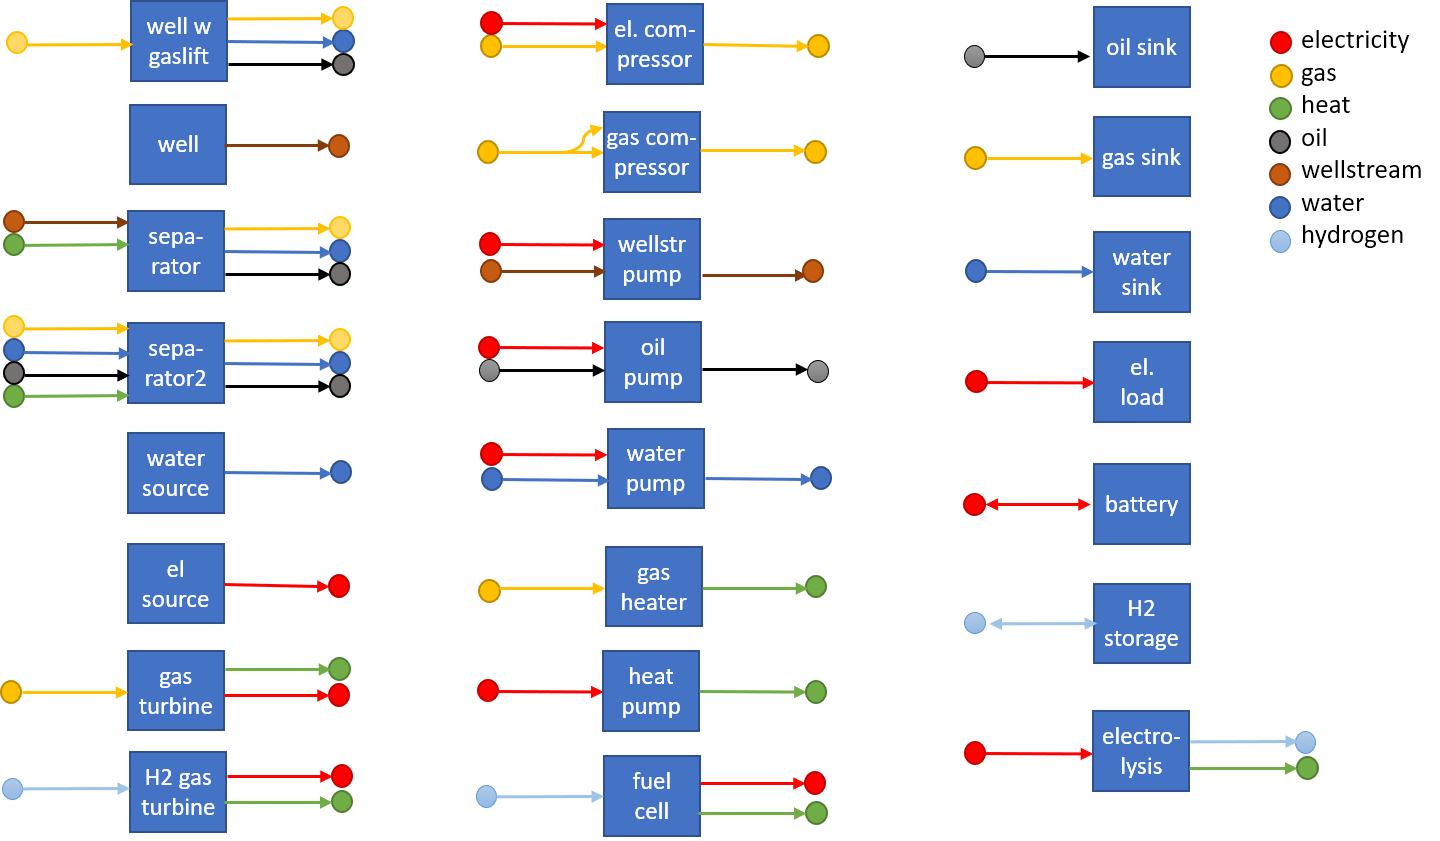
\includegraphics[width=\columnwidth]{./media/device_types.png}
		\caption{Illustration of some device types and their input/output energy streams }
		\label{fig:devicetypes}
\end{figure}



\subsection{Production well [well\_production]}

A production well is a petroleum source, with a natural well head pressure that allows a mixed liquid to flow up at a certain rate. Flow from multiple wells is combined in a manifold and fed into a separator.

\begin{itemize}
\item In: --
\item Out: wellstream
\item Parameters:
\begin{itemize}[noitemsep,topsep=0pt]
	\item $p_{natural}$,  wellhead natural pressure [MPa]
	\item $Q_\text{max}$, $Q_\text{min}$ [optional], wellstream max/min flow rate [Sm3/s]
	\item profile identifier (string ID) [optional], a time-varying profile that modifies $Q_\text{max}$
\end{itemize}
\end{itemize}

\medskip\noindent
Output terminal pressure equals natural pressure:
 \begin{equation}
 	p_{out}=p_{natural} 
 \end{equation}

Gas lift is not yet considered.





\subsection{Separator [separator]}

A separator splits the mixed liquid stream from the well into oil, gas and water in a separation process. 

\begin{itemize}
\item In: wellstream, heat, el
\item Out: oil, gas, water
\item Parameters:
\begin{itemize}[noitemsep,topsep=0pt]
	\item $ \eta _{el}$ electric demand as fraction of wellstream inflow [MJ/Sm3]
	\item $ \eta _{heat}$ heat demand as fraction of wellstream inflow [MJ/Sm3]
	\item output nominal pressure (gas, oil, water)
	\item $c$, wellstream composition factors
\end{itemize}
\end{itemize}



Flow out of separator is determined by wellstream flow in in and composition factors:
 \begin{align}
 Q_{out}^{gas} &=c_{gas}Q_{in}^{wellstream} \\
 Q_{out}^{oil} &=c_{oil}Q_{in}^{wellstream} \\
 Q_{out}^{water} &=c_{water}Q_{in}^{wellstream} 
 \end{align}
 %
Separator heat and power demands are assumed proportional to the well stream flow, 
with proportionality factors provided as input:
\begin{align}
	P_{in}^{el} 		&= \eta _{el}Q_{in}^{wellstream}\\
	P_{in}^{heat}	&= \eta _{heat}Q_{in}^{wellstream}
\end{align}
%
Output pressure is equal to nominal pressure specified for terminals:
\begin{align}
 p_{out}^{gas}		&=p_{out,0}^{gas} \\
 p_{out}^{oil}		&=p_{out,0}^{oil} \\
 p_{out}^{water}	&=p_{out,0}^{water} 
 \end{align}

\noindent 
\textit{Presently no dependence on input pressure is considered}



\subsection{Compressor [compressor\_el]}
A compressor is used to increase gas pressure. It may be driven by gas (see below) or electricity.


\begin{itemize}
\item In: gas, el
\item Out: gas
\item Parameters:
\begin{itemize}[noitemsep,topsep=0pt]
	\item $\eta_{is}$,  isentropic efficiency efficiency (example: 0.7)
	\item $T_1$, inlet temperature [K]
	\item $Q_0$, gas flow operating point used for linearisation
\end{itemize}
\end{itemize}






\medskip\noindent
Symbols used in the following description of compressors are defined in Table~\ref{tab:compressorsymbols}
Compressor power consumption can be computed from the work done compressing the gas, assuming the ideal gas law 
\begin{equation}
 	 pV^{k}=ZmRT, 
\end{equation}
where  \( k=\frac{c_{P}}{c_{V}} \)  is the specific heat ratio,  \( Z \)  is compressibility factor,  \( R \)  is the characteristic gas constant  \( m \)  is the amount of gas (mass),  \( V \)  is the volume,  \( p \)  is the pressure and  \( T \)  is the temperature. This expression together with the expression for work done in an adiabatic process,  \( dW=pdV \) , can be used to derive the compressor power consumption as:
\begin{equation}
	P_{compr}=\frac{\dot{m}}{ \eta _{is}}\frac{1}{k-1}ZRT_{1} \left[  \left( \frac{p_{2}}{p_{1}} \right) ^{\frac{k-1}{k}}-1 \right] 
		=c Q \left[  \left( \frac{p_{2}}{p_{1}} \right) ^{ \alpha }-1 \right] , 
\end{equation} 
where  \( \dot{m} \)  is the mass flow rate,  \(  \eta _{is} \)  is the isentropic efficiency, and subscripts 1 and 2 refer to inlet and outlet respectively, and we have defined
\begin{equation}
	c=\frac{ \rho _{s}}{ \eta _{is}}\frac{1}{k-1}ZRT_{1},~~ \alpha =\frac{k-1}{k}. 
\end{equation}


The mass flow is related to standard condition volumetric flow and energy flow via,  \( \dot{m}= \rho _{s}Q= \rho _{s}\frac{P}{CV} \) , where  \(  \rho _{s} \)  is the standard condition mass density and  \( CV \)  is the energy content. For natural gas,  \( k=1.27 \)  and  \( R=438\frac{J}{\text{kg K}} \) ,  \(  \rho _{s}=0.84\frac{kg}{m^{3}} \) . Assuming values  \(  \eta _{is}=0.7, T=300 K, Z=1, \)  and compression ratio  \( \frac{p_{2}}{p_{1}}=5  \) we get:
\begin{equation}
	P_{compr}
	=0.584 \frac{MJ}{Sm^{3}} \left[  \left( \frac{p_{2}}{p_{1}} \right) ^{0.21}-1 \right] Q
	=0.23\frac{MJ}{Sm^{3}} Q=\text{0.0059 P}. 
\end{equation} 
I.e. the compressor power consumption is 0.06$\%$  of the power content of the gas being compressed.


The power consumption depends non-linearly on flow rate and pressure (and temperature), so for the linear model, this needs to be simplified. Linearisation around operating points
\begin{equation}
	 p_{1}=p_{1}^{0}+ \Delta p_{1},~~p_{2}=p_{2}^{0}+ \Delta p_{2},~\dot{m}= \rho _{s}Q= \rho _{s} \left( Q^{0}+ \Delta Q \right) ,
\end{equation} 
gives
\begin{equation}
 \begin{split}
 P_{compr} & 
 	=c Q \left[  \left( \frac{p_{2}}{p_{1}} \right) ^{ \alpha }-1 \right] 
 \\ &
	=P_{compr}^{0}+\frac{ \partial P}{ \partial Q} \Delta Q+\frac{ \partial P}{ \partial p_{1}} \Delta p_{1}+\frac{ \partial P}{ \partial p_{2}} \Delta p_{2}+O \left(  \Delta ^{2} \right)  
 \\ & 
	=c Q^{0} \left[  \left( \frac{p_{2}^{0}}{p_{1}^{0}} \right) ^{ \alpha }-1 \right] +c \left(  \left( \frac{p_{2}^{0}}{p_{1}^{0}} \right) ^{ \alpha }-1 \right)  \Delta Q
	\\& \qquad +c \alpha Q^{0} \left( \frac{p_{2}^{0}}{p_{1}^{0}} \right) ^{ \alpha } \left( -\frac{ \Delta p_{1}}{p_{1}^{0}}+\frac{ \Delta p_{2}}{p_{2}^{0}} \right) +O \left(  \Delta ^{2} \right)  
 \\ & 
	=c  \left\{  \alpha  \left( \frac{p_{2}^{0}}{p_{1}^{0}} \right) ^{ \alpha }Q^{0} 
 	\left( \frac{p_{2}}{p_{2}^{0}}-\frac{p_{1}}{p_{1}^{0}} \right) 
 	+ \left(  \left( \frac{p_{2}^{0}}{p_{1}^{0}} \right) ^{ \alpha }-1 \right) Q \right\} 
 +O \left(  \Delta ^{2} \right) . 
 \end{split}
 \end{equation}
%
If pressure variations can be ignored, the linearised expression is identical to the full one:
\begin{equation}
	P_{compr}=c  \left(  \left( \frac{p_{2}^{0}}{p_{1}^{0}} \right) ^{ \alpha }-1 \right) Q
\end{equation}



\begin{table}[]
\caption{Symbols used for compressor description}
\label{tab:compressorsymbols}
\begin{tabular}{llp{12em}l}
\hline
symbol    		& unit   & description                                & value              \\
\hline
$R$         		& J/kg K & characteristig gas constant                & 438 (natural gas)  \\
$k=\frac{c_P}{c_V}$ & 1      & specific heat ratio of gas                 & 1.27 (natural gas) \\
$\eta_{is}$      & 1      & isentropic efficiency                      & 0.7                \\
$Z$         		& 1      & compressibility factor (Z=1 for ideal gas) & 1                  \\
$\rho_s$		& kg/Sm3 & gas density (standard conditions)          & 0.84 (natural gas) \\
\hline
\end{tabular}
\end{table}


Compressor power demand is a function of inlet/outlet pressure and flow, as described above:
 \begin{equation}
 	 P^{el}_{in}=P_{compr} 
\end{equation} 
Gas flow out is equal to gas flow in:
\begin{equation}
	 Q_{out}^{gas}=Q_{in}^{gas}
\end{equation} 
Outlet pressure is fixed at nominal value:
\begin{equation}
	p_{2}=p_{2}^{0} 
\end{equation}


\subsection{Compressor [compressor\_gas]}

A gas-driven compressor is like an electrically driven compressor, but with power demand supplied from the gas flowing through.


\begin{itemize}
\item In: gas
\item Out: gas
\item Parameters:
\begin{itemize}[noitemsep,topsep=0pt]
	\item $\eta_{is}$,  efficiency, including efficiency of converting gas energy content to work (so this value is less for gas compressor than for an electric compressor) (example: 0.7)
	\item $T_1$, inlet temperature [K]
	\item $Q_0$, gas flow operating point used for linearisation
\end{itemize}
\end{itemize}



\medskip\noindent
Power demand  \( P_{compr} \)  is computed in the same way as for electric compressor.

The gas output equals the input minus the self-consumption:
 \begin{equation}
 	Q_{out}^{gas}=Q_{in}^{gas}-\frac{P_{compr}}{CV} 
\end{equation}



\subsection{Water pump [pump\_water]}

A water pump may be used either to pump water up from a water reservoir, or into an injection well. Water injection wells are used to increase/maintain the reservoir pressure, which in turn is needed to extract petroleum.  


\begin{itemize}
\item In: water, el
\item Out: water
\item Parameters:
\begin{itemize}[noitemsep,topsep=0pt]
	\item $\eta$,  pump efficiency (example: 0.8)
\end{itemize}
\end{itemize}

\medskip\noindent
Electric power is needed by a pump to increase water pressure and can be computed considering the work needed to move the liquid up a pressure gradient. The power is work per time, so assuming constant flow-rate (incompressible fluid):
 \begin{equation}
 \begin{split}
 P &=\frac{d}{dt}W
	 =\frac{d}{dt} \int _{}^{}Fds
	 =\frac{d}{dt} \int _{}^{}pAds
	 =\frac{d}{dt} \int _{}^{}pdV
	 \\& 
	 = \int _{}^{}\frac{d}{dt}pQdt
	 =Q \int _{p_{1}}^{p_{2}}dp
	 =Q \left( p_{2}-p_{1} \right)  
 \end{split}
 \end{equation}


Accounting for the efficiency of the pump we therefore have
 \begin{equation} 
 	\eta P_{in}^{el}=P=Q \left( p_{2}-p_{1} \right) . 
 \end{equation}
%
Expanding around operating points  
\begin{equation}
 p_{1}=p_{1}^{0}+ \Delta p_{1},~~p_{2}=p_{2}^{0}+ \Delta p_{2}, Q=Q^{0}+ \Delta Q, 
 \end{equation} 
 this becomes
%
\begin{equation}
 \begin{split}
 P &=Q^{0} \left( p_{2}^{0}-p_{1}^{0} \right) 
 		+ \left( Q-Q^{0} \right)  \left( p_{2}^{0}-p_{1}^{0} \right) 
	\\& \qquad
 		+Q^{0} \left( ~p_{2}-p_{2}^{0} \right) 
 		-Q^{0} \left( p_{1}-p_{1}^{0} \right) 
 		+O \left(  \Delta ^{2} \right)  
	\\ &
	=Q \left( p_{2}^{0}-p_{1}^{0} \right) +Q^{0} \left( ~p_{2}-p_{2}^{0} \right) 
		-Q^{0} \left( p_{1}-p_{1}^{0} \right) 
		+O \left(  \Delta ^{2} \right)  
%	\\ &
%	=Q \left( p_{2}^{0}-p_{1}^{0} \right) +Q^{0} \left( ~p_{2}-p_{1} \right)
%		-Q^{0} \left( p_{2}^{0}-p_{1}^{0} \right) 
%		+O \left(  \Delta ^{2} \right)  
 \end{split}
 \end{equation}
%
Considering that the outlet pressure is determined by the reservoir pressure and fixed ($p_{2}=p_{2}^{0}$), we get the linear relationship,
 \begin{equation} 
 \eta P_{in}^{el}= P
 	= \left[ Q \left( p_{2}^{0}-p_{1}^{0} \right) +Q^{0} \left( p_{1}^{0}-p_{1} \right)  \right].  
 \end{equation}


Assuming that the pressure deviations are small, we can ignore the second term. Therefore, the electric power demand is proportional to water flow:
 \begin{equation}
 \eta P_{in}^{el}=Q_{in}^{water} \left( p_{2}^{0}-p_{1}^{0} \right)  
 \end{equation}



\subsection{Oil pump [pump\_oil]}
An oil pump is as pump that increases oil pressure for transport through pipelines.

\begin{itemize}
\item In: oil, el
\item Out: oil
\item Parameters:
\begin{itemize}[noitemsep,topsep=0pt]
	\item $\eta$,  efficiency
\end{itemize}
\end{itemize}


\textit{As for water pumps, we pressure ignore inlet and outlet pressure variations (deviations from nominal values)}

Flow out equals flow in
\begin{equation}
	Q_{out}^{oil}=Q_{in}^{oil}
\end{equation}
Pump power demand is proportional to energy flow and (nominal) pressure difrerence
\begin{equation}
	\eta P^{el}_{in} = \eta Q_{in}^{oil}(p^0_2-p^0_1),
\end{equation}
where $p^0_1$ and $p^0_2$ are nominal pressure levels at inlet and outlet respectively.


\subsection{Gas heater [gasheater]}
A gas heater produces heat from burning gas.

\begin{itemize}
\item In: gas
\item Out: heat
\item Parameters:
\begin{itemize}[noitemsep,topsep=0pt]
	\item $\eta_{heat}$,  efficiency
\end{itemize}
\end{itemize}

Heat output equals heating efficiency times gas consumption:
\begin{equation}
	P_{out}^{heat}= \eta _{heat}P_{in}^{gas}
\end{equation}



\subsection{Heat pump and electric boiler [heatpump]}

A heat pump or boiler converts electrical energy to heat using an external heat source. The electric heating efficiency for air-to-air heat pumps is typically around  \(  \eta _{heat}=3 \) .\  The temperature dependence is not modelled.

\begin{itemize}
\item In: el
\item Out: heat
\item Parameters:
\begin{itemize}[noitemsep,topsep=0pt]
	\item $\eta_{heat}$,  efficiency
\end{itemize}
\end{itemize}

Heat output equals electric power times efficiency:
\begin{equation}
	P_{out}^{heat}= \eta _{heat}P_{in}^{el}
\end{equation}



\subsection{Gas turbine [gasturbine]}
A gas turbine generator converts natural gas to electric power and heat.

\begin{itemize}
\item In:gas
\item Out: el
\item Parameters:
\begin{itemize}[noitemsep,topsep=0pt]
	\item $\eta_{heat}$,  output heat as fraction of power output
	\item 	$A$, $B$, fuel consumption parameters
\end{itemize}
\end{itemize}


\medskip\noindent

Fuel consumption  \( Q_{in}^{gas} \)  is assumed to be a linear function of the electrical power output  \( P_{out}^{el} \) :
\begin{equation}
	 \frac{Q_{in}^{gas} CV}{P_{\max }}=A\frac{P_{out}^{el}}{P_{\max }}+B 
\end{equation}


To determine typical $A$ and $B$ parameter values, we use
emission factors found in the literature.\footnote{ MA Gonzalez-Salazara, T Kirstena, L Prchlik, Review of the operational flexibility and emissions of gas- and coal-fired power plants in a future with growing renewables Ren Sust Energy Rev. (2018), https://doi.org/10.1016/j.rser.2017.05.278  }
%
At maximum power (\( P_{out}^{el}=P_{\max } \)), the fuel consumption should be about  \( A+B \) =1/0.347 (efficiency about 34.7$\%$ ). At minimum load (ca 20$\%$  loading), the efficiency should be about 20$\%$ , i.e.  \( \frac{0.2A+B}{0.2}=0.2 \) . Together these two conditions give A=2.35, B=0.53. Schematics of fuel characteristics of gas turbines are shown in Figure~\ref{fig:gasturbine_fuel}.

The specific fuel efficiency is the gas fuel usage (in MW) times the CO2 content (kg/MWh) divided by the electric output (in MW). The CO2 content of natural gas combusted on the Norwegian continental shelf is%
\footnote{T Sandmo, SSB Documents 2016/22, https://www.ssb.no/natur-og-miljo/artikler-og-publikasjoner/the-norwegian-emission-inventory-2016 (Table B1) } 
2.34 kgCO2/Sm3 (using density and energy content factors, this equals 2.03 kgCO2/kg\textsubscript{gas} 
or 211 kgCO2/MWh\textsubscript{gas}). 



Power output is non-zero only if gas turbine is running:
\begin{equation}
	 P_{out}^{el} \leq yP_{\max },
\end{equation}
where  $y$ is a binary variable that is 0 if turbine is not running and 1 if the turbine is running.

Heat output is given as gas fuel consumption (energy content) times a a heat fraction parameter:
 \begin{equation}
% 	P_{out}^{heat}= \eta _{heat}P^{el}_{in}
	P_{out}^{heat}= \eta _{heat}Q_{in}^{gas} CV
\end{equation}

\begin{figure}[]
\centering
		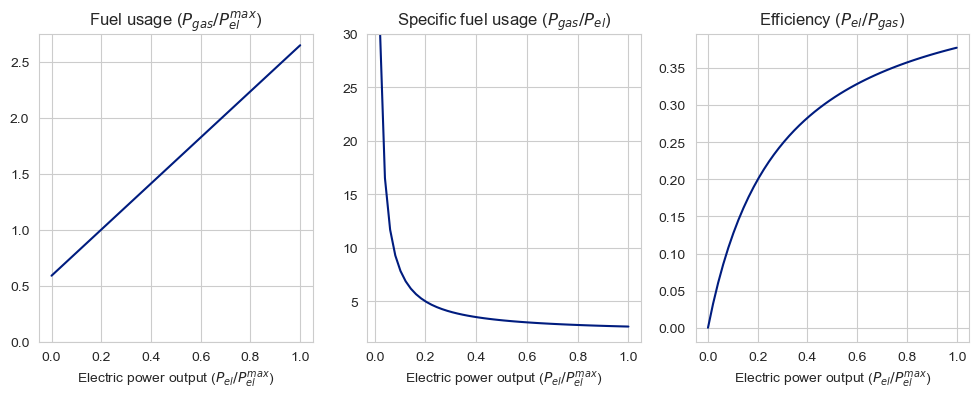
\includegraphics[width=\columnwidth]{./media/gt_fuel_curves.png}
		\caption{Gas turbine fuel characteristics (schematic, for A=2.35, B=0.53)}
		\label{fig:gasturbine_fuel}
\end{figure}



\subsection{Source water [source\_water]}

Water source. 
This external source may be associated with a time-series that specifies available power and determines the maximum output value.

\begin{itemize}
\item In: --
\item Out: water
\item Parameters: 
\begin{itemize}[noitemsep,topsep=0pt]
	\item $p_{natural}$ , natural pressure (MPa)
\end{itemize}
\end{itemize}

\medskip\noindent
The output pressure equals the natural pressure,
\begin{equation}
	p^{water}_{out} = p_{natural}
\end{equation}



\subsection{Source el [source\_el]}

Electric power source. This may be a wind turbine, diesel generator, solar power generator or similar – something that generates electricity from an external source. 
This external source may be associated with a time-series that specifies available power and determines the maximum output value.

\begin{itemize}
\item In: --
\item Out: el
\item Parameters: --
\end{itemize}


\subsection{Electrical battery [storage\_el]}
Electrical storage can absorb electrical power (charging) or supply electrical power (discharging), with some losses indicated by the cycle efficiency parameter.

\begin{itemize}
\item In:el
\item Out: el
\item Parameters:
\begin{itemize}[noitemsep,topsep=0pt]
	\item $2\eta$,  cycle efficiency
	\item $E_{max}$,  energy storage capacity
\end{itemize}
\end{itemize}

\medskip\noindent
Energy balance of the storage:
\begin{equation}
	 \left[  \eta P_{in}^{el}-\frac{1}{ \eta }P_{out}^{el} \right]  \Delta t=E_{t}-E_{t-1}, 
\end{equation}
where  $\Delta t$  is the time-step length.


Energy storage is limited by lower and upper bounds:
 \begin{equation}
 0 \leq E_{t} \leq E_{\max } 
 \end{equation}
 
Charging and discharging limits:
 \begin{equation}
 P_{in}^{el} \leq P_{\max } , \qquad
 P_{out}^{el} \leq P_{\max } .
 \end{equation}





\subsection{Water sink [sink\_water]}

A  water sink, either for water disposal or water injection. The pressure is specified by the parameters of the water pipe (edge) connecting to the water sink.

\begin{itemize}
\item In: water
\item Out: --
\item Parameters:
\begin{itemize}[noitemsep,topsep=0pt]
	\item $Q_{avg}$  (optional), water flow required average (Sm3/s)
	\item $V_{\max }$ (optional),  water flow buffer size (allowing flexibility) (Sm3/s h) 
\end{itemize}
\end{itemize}

\medskip\noindent
\textit{Flexible} water injection is modelled by introducing a buffer of limited size $V_{\max }$ that decouples the long-term required average water flow  $Q_{avg}$ from the actual water flaw at a given time.
%
Change in volume buffer level  $V_{t}$  equals water in minus required average flow  \( Q_{avg} \) 
 \begin{equation}
 	\left[ Q_{in}^{water}-Q_{avg} \right]  \Delta t=V_{t}-V_{t-1}, 
 \end{equation}
where  $\Delta t$ is the time-step length.
%
The buffer level is limited by lower and upper bounds
 \begin{equation}
	 -\frac{V_{\max }}{2} \leq V_{t} \leq \frac{V_{\max }}{2} 
 \end{equation}





\subsection{Gas sink [sink\_gas]}
Generic gas load (or export point)

\begin{itemize}
\item In:gas
\item Out: --
\item Parameters: --
\end{itemize}


\subsection{Oil sink [sink\_oil]}

Generic oil load (or export point)

\begin{itemize}
\item In:oil
\item Out: --
\item Parameters: --
\end{itemize}


\textbf{Constraint:}
Device power equals oil in
 \[ P_{device}=P_{oil}^{gas} \] 


\subsection{Electrical load [sink\_el]}

Generic electrical load.

\begin{itemize}
\item In:el
\item Out: --
\item Parameters: --
\end{itemize}



\subsection{Heat sink [sink\_heat]}

Generic heat load.

\begin{itemize}
\item In:heat
\item Out: el
\item Parameters: --
\end{itemize}


\subsection{Device types not yet implemented}
Device types that may be implemented later:
\begin{itemize}
	\item Heat storage
	\item Electrolysis (el to H2)
	\item fuel cell (H2 to el)
	\item H2 turbine (H2 to el/heat)
	\item H2 storage
	\item gas-to-fuel (H2+CO2)
	\item heat demand determined by thermodynamic equations (heat storage, heat loss function of temperature difference, max/min temperature)
\end{itemize}

\section{Other constraints}

 
 
\subsection{Start-up time}

Devices may be specified with a start-up delay, meaning that once turned on, some time is required before power can be ramped up. This is relevant at least for gas turbines. 
Simple cycle gas turbines may have a start-up delay of 10 minutes, while combined cycle gas turbines about 30 minutes.

Four binary variables are used to encode the logic for startup and shutdown of gas turbine generators where it takes some time from activation to power output to the system: 
\begin{itemize}
\item isStarting: 1 when device is activated, 0 otherwise
\item isPrep: 1 when device is in startup preparation phase (after activation), 0 otherwise
\item isOn: 1 when device is online, 0 otherwise (denoted $y$ above)
\item isStopping: 1 when device is shut down, 0 otherwise
\end{itemize}

\medskip\noindent
The equtions linking these are:
\begin{equation}
	isOn(t) - isOn(t-1) = isStarting(t-tDelay) - isStopping(t),
\end{equation}
\begin{equation}
	isPrep(t)  = \sum_{\tau=0}^{tDelay-1} isStarting(t-\tau),
\end{equation}
where $tDelay$ is the startup time measured in timesteps.
For the first timesteps when $t<tDelay$ these equations are modified to include the results from the previous rolling horizon.


\subsection{Spinning reserve requirement}
Spinning reserve capacity is usually required to cover unforeseen variation in power demand and supply.

The reserve contribution from a single generating unit is computed as 
\begin{equation}
	R_{gen}(t) = p(t) P_{max} - P_{out}(t),
\end{equation}
where $p(t)$ is a profile that gives the available power relative to the installed capacity.

For a load, the reserve capacity contribution is the part of the load which can be reduced (if any):
\begin{equation}
	R_{load} \left( t \right) = f^{reduction}P_{in}(t), 
\end{equation}
where  \( f_{i}^{reduction} \)  is a factor (input parameter) that specifies which fraction of the load that can be reduced. 
If the load cannot be reduced, this factor is zero. If the load can be turned off completely, it is one.

For energy storage devices, the reserve is given by the mimimum of the available energy and the power rating:
\begin{equation}
	R_{stor}(t) = \min{P_{max}, \frac{E(t)}{\Delta t}},
\end{equation}
where $\Delta t$ is the length of each timestep. For example, if the timesteps are 5 min=5/60 hours, and the energy level is $E(t)=2$~MWh, then the available power is $P=\frac{2}{5/60}$~MW = 24 MW. 
However, if the battery power rating is e.g. 4 MW, only 4 MW can be output.

\textit{For a battery, the available power is in reality limited not just by the maximum power, but also by the energy stored in the battery. This is not included at present. Possibly, this could be included in a linear way by computing an effective capacity profile from the battery energy scheduling from the previous timestep optimisation}.

The overall reserve capacity is then
\begin{equation}
	R=  \sum R_{gen} + \sum R_{load}  \ \sum R_{stor} . 
\end{equation}
And the resrve requirement (optimisation constraint) is
\begin{equation}
	R(t) \ge R_{min}(t)
\end{equation}


\subsection{Backup power requirement}
In addition or instead of defining a reserve requirement, it is possible to specify a backup power requirement. This is simlar to the reserve requirement, but instead of considering variations in demand or power availability, it considers generator trips.
In the case of such a trip, or fault, on a power supply unit, online backup capacity may be required to cover the lost supply – either by ramping up other supply units, by reducing power consumption by loads, or by shedding loads.

The main difference from the reserve requirement described above is that this considers \emph{fault} situations, and therefore the reserve contribution from the generator itself must be excluded. For example, if two 20 MW generators are running at 11 MW to supply a 22 MW load, the reserve is 18 MW, but if one of them trips, the other gas turbine can only increase by 9 MW, not enough to cover the lost supply. That is, either we need a third generator online, or we must be able to reduce or shed loads.


The overall backup capacity to take over in case generator $i$ trips, \emph{excluding the contribution from the device itself}  is:
\begin{equation}
 	R_{i}=  \sum _{j \neq i}^{} \left[ R_{gen}^j(t) +R_{load}^j(t) +R_{stor}^j(t) \right] . 
\end{equation}
The backup power requirement sets a lower limit for how much power loss is allowed ($P^{loss}_{max}$) in case of a trip and sudden loss of $P_i$ power from generator $i$: 
 \begin{equation}
 	R_{i}   \geq P_i - P^{loss}_{max}.
 \end{equation}



\section{Input data}
The input data consists of a YAML file containing specifications of all elements (nodes, edges, devices) included, how they are connected (network topology) and parameters for each element. A separate file (XLSX or HD5) containts time-series profiles.

\subsection{YAML file -- elements, topology, and parameter values}

The YAML file includes the following elements:
\begin{itemize}
\item paramParameters -- global parameters
\item paramCarriers -- energy/mass flow carriers and their parameters
\item paramDevice -- devices and their parameters
\item paramEdge -- edges (pipes/conductors) and their parameters
\item paramNode -- nodes and their parameters
\end{itemize}


\begin{table}[h]
\caption{Profiles input data}
\begin{tabular}{lll}
	\hline
	header & type & description \\
	\hline
	timestep & int & timestep identifier (0,1,2,...) \\
	time & datetime & timestamp (optional, this column is ignored) \\
	comment & string & comment (optional, this column is ignored) \\
	profiles & float & one column per profile (header is profile identifier)\\
\end{tabular}
\end{table}

%\FloatBarrier

\section{Examples}

Examples showing how to use the simulation tool are provided together with the program code at
\url{https://bitbucket.org/harald_g_svendsen/oogeso}.





\printbibliography
\end{document}

